\documentclass[10pt]{article}
% biber (para que funcione el comp de vim)
%%% Cargo paquetes{{{
%% Para buscar documentacion de paquetes: http://texdoc.net/


%% Lenguaje{{{
\usepackage[utf8]{inputenc} % para poder usar tildes
\usepackage[spanish]{babel} % para escribir en español
%}}}


%% Formato{{{
% Fuente
\usepackage[]{times}

% Pagina
\usepackage[]{geometry} %Para definir donde se ubica el texto
\geometry{a4paper,textwidth={17cm},textheight={23cm},left={2cm},top={2.5cm},}

% Encabezado y Pie de pagina
\usepackage[]{fancyhdr}
\pagestyle{fancy}
\renewcommand{\headrulewidth}{0pt} % para que no haya linea decorativa en el header.

% Columnas
\usepackage[]{multicol} %Para poder usar columnas
\setlength{\columnsep}{1cm} %Separacion entre columnas de 1 cm

% Secciones{{{
\usepackage[]{titlesec} % Da formato a secciones
% Seccion
\titleformat{\section}
{\normalfont\LARGE\bfseries\MakeUppercase}{\thesection.}{.3em}{}
\titlespacing*{\section}{0cm}{0.25cm}{0.15cm}

% Subseccion
\titleformat{\subsection}
{\normalfont\Large\bfseries}{\thesubsection.}{.3em}{}
\titlespacing*{\subsection}{.15cm}{0.2cm}{0.1cm}

%Subsubseccion
\titleformat{\subsubsection}
{\normalfont\large\bfseries}{\thesubsubsection.}{.3em}{}
\titlespacing*{\subsubsection}{0.25cm}{0.15cm}{0.05cm}

\titleformat{\caption}
{\normalfont\large\bfseries}{\thesubsubsection.}{.3em}{}
\titlespacing*{\subsubsection}{0.25cm}{0.15cm}{0.05cm}
%}}}

% Para que las listas numeradas acepten opciones
\usepackage[]{enumerate} 



%  Mas opciones de formato para ecuaciones
\usepackage[]{amsmath}
\usepackage[]{amsfonts}%Requerido por amsmath
%}}}


%% Figuras y tablas{{{
\usepackage[]{graphicx}
\usepackage[space]{grffile} %Por si nombre de archivo tiene espacios
\usepackage[]{float} %Para poder usar [H] para poner fig en cols

\addto\captionsspanish{\def\tablename{Tabla}} % Cambiar ``cuadro'' por ``Tabla'' en captions
%}}}


%% Bibliografia{{{
\usepackage[backend=biber]{biblatex}
%}}}


%% Otros{{{
\usepackage[]{authblk}    % Para definir afiliaciones de autores
\renewcommand\Authsep{, }
\renewcommand\Authand{ y }
\renewcommand\Authands{ y }
\setlength{\affilsep}{0.5cm}


\usepackage[]{verbatim} % Para poder comentar por bloques
\usepackage[]{lipsum} % Para rellenar con texto
\usepackage[]{hyperref} % Para usar hipervinculos
%}}}

%}}}
%% Redefiniciones para dar formato{{{

% Abstract
\renewenvironment{abstract}{
	\noindent\hfill\begin{minipage}{\textwidth}
	Abstract --- \itshape}
	{\par\end{minipage}\vspace{1cm}}

% Captions(Epigrafes)
\usepackage[font=small,skip=0.3cm,tableposition=top,figureposition=bottom]{caption}
% para que la fuente de un epigrafe no tenga el mismo tamaño que el cuerpo del texto, tambien le indico donde va a estar para cada caso
%}}}

%% Mis commandos/definiciones{{{
\newcommand{\email}[1]{\texttt{\href{mailto:#1}{#1}} }

\newcommand{\titulo}[1]{\title{\Large\bfseries\MakeUppercase{#1}} }
\newcommand{\autor}[1]{\author{\bfseries\MakeUppercase{#1}} }
\newcommand{\materia}[1]{\newcommand{\materiavar}{#1}}
\newcommand{\fecha}[1]{\newcommand{\fechavar}{#1}}

\fancypagestyle{titlestyle}{
	\fancyhead[R]{\fechavar}
	\fancyhead[L]{\materiavar}
}
%}}}


%%% Opciones Generales del documento%{{{
\titulo{Report Format of Acoustic Laboratory}
\autor{Thomas C. Signal}
\affil{Ingeniería de Sonido, Universidad Nacional de Tres de Febrero \par \email{tsignal@gmail.com}}

\fecha{}
\date{} %Dejar blanco para que no aparesca en el titulo
\materia{Acoustic Laboratory}

\graphicspath{{img/}} %Defino carpeta para figuras
\addbibresource{biblio.bib}
%}}}




\begin{document}%{{{

\noindent{\begin{minipage}{\textwidth}
	\maketitle
	\thispagestyle{titlestyle}
\end{minipage}}


\pagestyle{fancy}
\fancyhf{}
\fancyfoot[R]{\thepage}
   

\begin{abstract}
En este trabajo se analiza la medición experimental de algunas características de los parlantes, en particular: la sensibilidad, la curva de impedancia, la respuesta en frecuencia, la directividad y los parámetros de Thiele-Small. Se describen dos métodos de medición, uno analógico y otro digital. Luego se presentan los resultados obtenidos de forma gráfica para permitir su análisis. Por último, se realizan sugerencias para mejorar los resultados sin la necesidad de grandes modificaciones a los métodos
\end{abstract}


%\begin{comment}
	
\begin{multicols*}{2} % Pongo el '*' para que no terminen parejas

\section{Introduction}


\subsection{Susbsec}
	%\lipsum{}
	\subsubsection{Subsubseccion}


	%\lipsum{}
	kk


sdhahask
\begin{figure}[H]
	\centering
	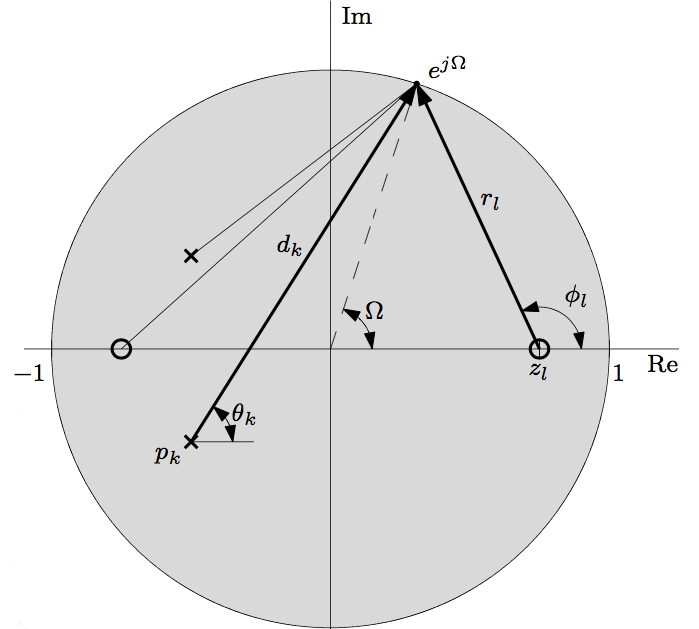
\includegraphics[width=\linewidth]{test.png}
	\caption{Esta es la figura.}
	\label{fig:test}
\end{figure}

casa

	%\lipsum{}
\begin{table}[H]
	\centering
	\caption{La tabla}
	\label{tab:la}
	\begin{tabular}{|c|c|c|c|}
	\hline
		Parámetro & Analógica & Digital & Datasheet \\
		\hline
		$f_{s}[Hz]$ & 165 & 168.4 & 130\\
		\hline
		$R_{e}[\Omega]$ & 4.9 & 5.1 & 5.7\\
		\hline
		$Q_{es}$ & 0.46 & 0.57 & 0.49\\
		\hline
		$Q_{ms}$ & 4.49 & 4.66 & 3.7\\
		\hline

	\end{tabular}

\end{table}



dklja
jdklsajs


kjdasjdklas

	ajsgdjsgdhs \cite{x6MD_man}.


\printbibliography

	\AtEndDocument{}
\end{multicols*}


\end{document}



%}}}
